\documentclass{standalone}

% graphics
\usepackage{tikz}
\usepackage{pgfplots}
\usepackage{siunitx}

\begin{document}

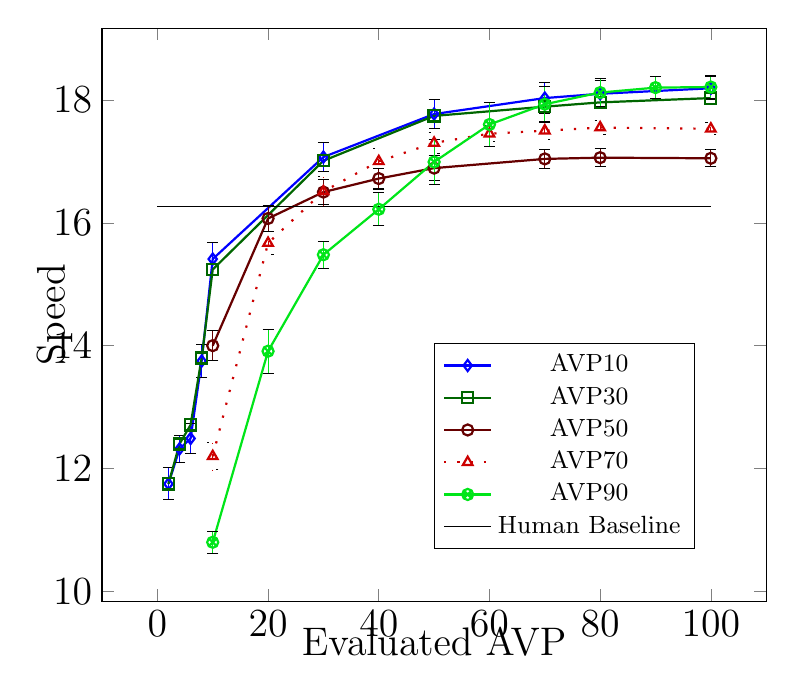
\begin{tikzpicture}[scale=1]
  \pgfplotsset{
      scale only axis,
      every x tick label/.append style={font=\Large},
      every y tick label/.append style={font=\Large},
	legend style={at={(0.5,0.45)},anchor=north west}
  }

\begin{axis}[
    legend style={font=\small},
	ylabel={\Large Speed},
	x label style={at={(axis description cs:0.5,-0.03)},anchor=north},
	y label style={at={(axis description cs:-0.030,0.5)}, anchor=south},
	xlabel={\Large Evaluated AVP},
]


% trained on avp=10 
% dashdotdotted,
\addplot[mark=diamond, thick, mark options={solid, fill=blue!40, mark size=2 pt}, draw=blue, error bars/.cd, y dir=both, y explicit] table [x=a, y=b, y error=c] {
a	b   	c
2 11.75 0.26
4 12.32 0.22
6 12.49 0.24
8 13.75 0.27
10 15.41 0.27
30 17.07 0.24
50 17.77 0.24
70 18.03 0.25
80 18.10 0.21
100 18.19 0.19
};
\label{AVP10}

% trained on avp=30
% error bars/.cd, y dir=both, y explicit,
\addplot[mark=square, thick, mark options={solid, fill=green!60, mark size=2 pt}, draw=black!60!green] table [x=a, y=b] {
a	b   	c
2 11.75 0.31
4 12.40 0.28
6 12.71 0.29
8 13.80 0.26
10 15.24 0.28
30 17.01 0.26
50 17.74 0.26
70 17.89 0.22
80 17.96 0.23
100 18.03 0.21
};
\label{AVP30}  

%densely dashed, 
\addplot[mark=o, thick, mark options={solid, fill=black!60!red, mark size=2pt}, draw=black!60!red, error bars/.cd, y dir=both, y explicit] table [x=a, y=b, y error=c] {
a	b   	c
10 14.00 0.24
20 16.07 0.21
30 16.50 0.20
40 16.72 0.17
50 16.89 0.20
70 17.04 0.15
80 17.06 0.15
100 17.05 0.14
};
\label{AVP50}

%densely dashed, 
\addplot[mark=triangle, thick, loosely dotted, mark options={solid, fill=red!60, mark size=2pt}, draw=black!20!red, error bars/.cd, y dir=both, y explicit] table [x=a, y=b, y error=c] {
a	b   	c
10 12.20 0.22
20 15.67 0.19
30 16.51 0.24
40 17.00 0.21
50 17.30 0.17
60 17.45 0.13
70 17.50 0.14
80 17.55 0.12
100 17.53 0.10
};
\label{AVP70}

%densely dashed, 
\addplot[mark=otimes, thick, mark options={solid, fill=red!60, mark size=2pt},
draw=blue!10!green, error bars/.cd, y dir=both, y explicit] table [x=a, y=b, y error=c] {
a	b   	c
10 10.80 0.18
20 13.91 0.36
30 15.48 0.22
40 16.22 0.27
50 16.99 0.36
60 17.60 0.36
70 17.93 0.29
80 18.12 0.23
90 18.20 0.18
100 18.21 0.18
};
\label{AVP90}


\addplot[mark=none, black, samples=200] coordinates {(0,16.27) (100,16.27)};{};\label{Baseline}

\addlegendimage{/pgfplots/refstyle=AVP10}
\addlegendentry{AVP10}

\addlegendimage{/pgfplots/refstyle=AVP30}
\addlegendentry{AVP30}

\addlegendimage{/pgfplots/refstyle=AVP50}
\addlegendentry{AVP50}

\addlegendimage{/pgfplots/refstyle=AVP70}
\addlegendentry{AVP70}

\addlegendimage{/pgfplots/refstyle=AVP90}
\addlegendentry{AVP90}

\addlegendimage{/pgfplots/refstyle=Baseline}
\addlegendentry{Human Baseline}




\end{axis}
\end{tikzpicture}

\end{document}

